
\documentclass{standalone}
\usepackage{xcolor}
\usepackage{pgfplots}
\pgfplotsset{compat=1.18}

\begin{document}

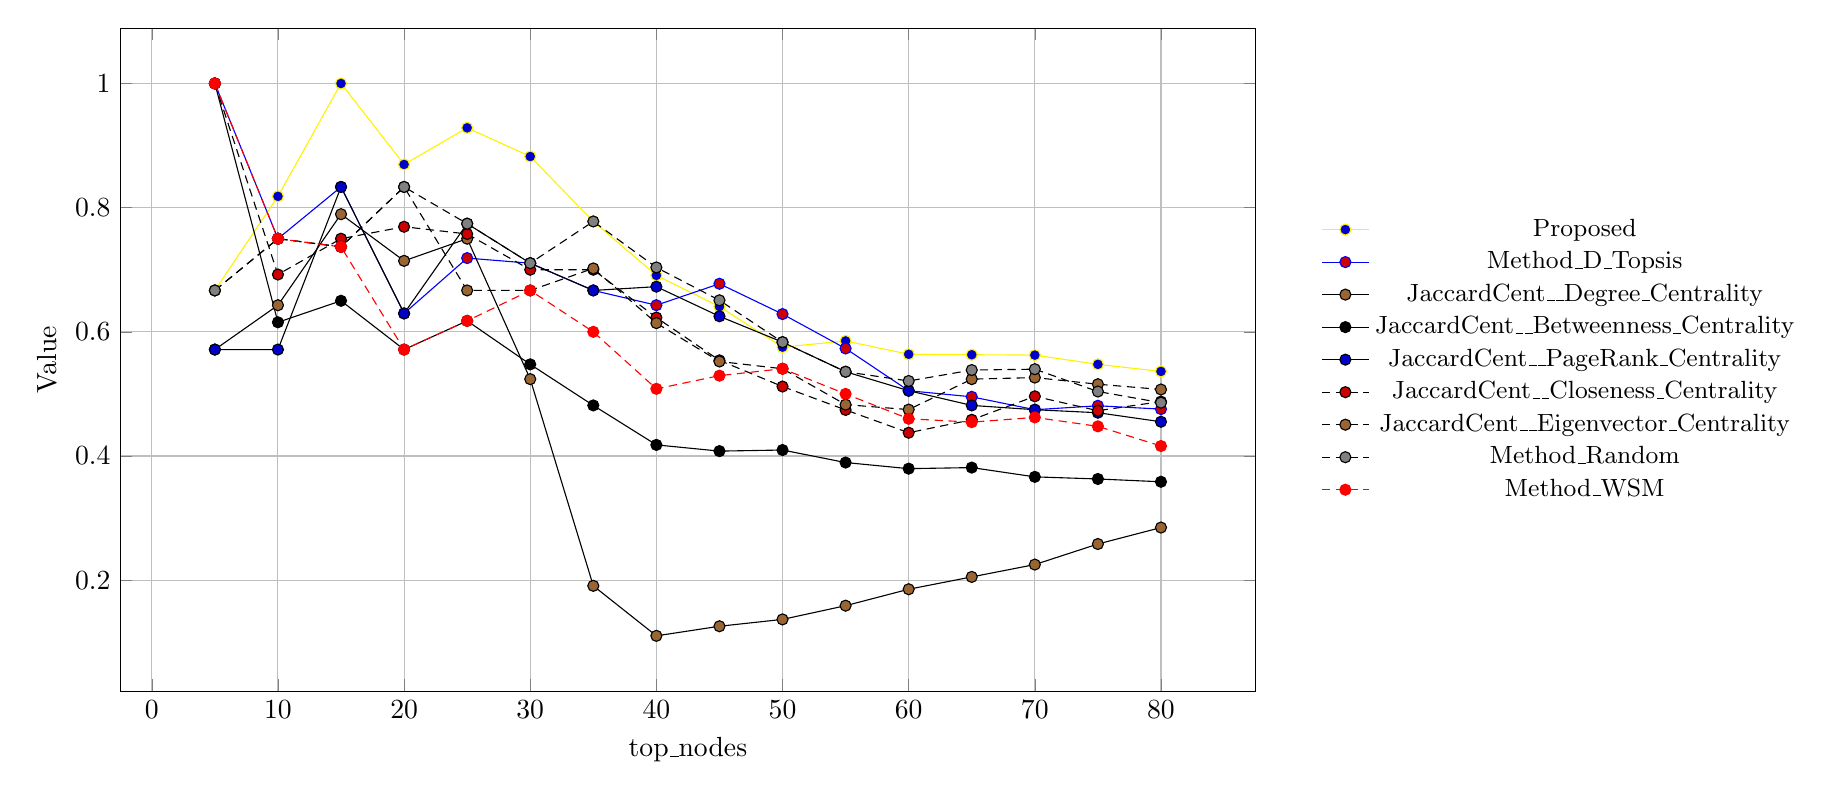
\begin{tikzpicture}
\begin{axis}[
    width=16cm,
    height=10cm,
    xlabel={top\_nodes},
    ylabel={Value},
    grid=major,
    legend style={
        at={(1.05,0.5)},
        anchor=west,
        font=\small,
        draw=none,
        cells={align=left},
    },
]
% Proposed
\addplot+[color=yellow, mark=*] coordinates {
(5.0,0.6666666666666666) (10.0,0.8181818181818182) (15.0,1.0) (20.0,0.8695652173913043) (25.0,0.9285714285714286) (30.0,0.8823529411764706) (35.0,0.7777777777777778) (40.0,0.6909090909090909) (45.0,0.640625) (50.0,0.5753424657534246) (55.0,0.5853658536585366) (60.0,0.5638297872340425) (65.0,0.5631067961165048) (70.0,0.5625) (75.0,0.5476190476190477) (80.0,0.5362318840579711) };
\addlegendentry{Proposed}

% Method\_D\_Topsis
\addplot+[color=blue, mark=*] coordinates {
(5.0,1.0) (10.0,0.75) (15.0,0.8333333333333334) (20.0,0.6296296296296297) (25.0,0.71875) (30.0,0.7105263157894737) (35.0,0.6666666666666666) (40.0,0.6428571428571429) (45.0,0.6774193548387096) (50.0,0.6285714285714286) (55.0,0.573170731707317) (60.0,0.5051546391752577) (65.0,0.4953271028037383) (70.0,0.4745762711864407) (75.0,0.4809160305343511) (80.0,0.4755244755244755) };
\addlegendentry{Method\_D\_Topsis}

% JaccardCent\_\_Degree\_Centrality
\addplot+[color=black, mark=*] coordinates {
(5.0,0.5714285714285714) (10.0,0.6428571428571429) (15.0,0.7894736842105263) (20.0,0.7142857142857143) (25.0,0.75) (30.0,0.5238095238095238) (35.0,0.1909090909090909) (40.0,0.1103752759381898) (45.0,0.1258278145695364) (50.0,0.1368653421633554) (55.0,0.1589403973509933) (60.0,0.1854304635761589) (65.0,0.2052980132450331) (70.0,0.2251655629139073) (75.0,0.2582781456953642) (80.0,0.2847682119205298) };
\addlegendentry{JaccardCent\_\_Degree\_Centrality}

% JaccardCent\_\_Betweenness\_Centrality
\addplot+[color=black, mark=*] coordinates {
(5.0,1.0) (10.0,0.6153846153846154) (15.0,0.65) (20.0,0.5714285714285714) (25.0,0.6176470588235294) (30.0,0.5476190476190477) (35.0,0.4814814814814814) (40.0,0.417910447761194) (45.0,0.4078947368421052) (50.0,0.4096385542168674) (55.0,0.3894736842105263) (60.0,0.3796296296296296) (65.0,0.3813559322033898) (70.0,0.366412213740458) (75.0,0.363013698630137) (80.0,0.3584905660377358) };
\addlegendentry{JaccardCent\_\_Betweenness\_Centrality}

% JaccardCent\_\_PageRank\_Centrality
\addplot+[color=black, mark=*] coordinates {
(5.0,0.5714285714285714) (10.0,0.5714285714285714) (15.0,0.8333333333333334) (20.0,0.6296296296296297) (25.0,0.7741935483870968) (30.0,0.7105263157894737) (35.0,0.6666666666666666) (40.0,0.6727272727272727) (45.0,0.625) (50.0,0.5833333333333334) (55.0,0.5357142857142857) (60.0,0.5051546391752577) (65.0,0.4814814814814814) (70.0,0.4745762711864407) (75.0,0.4696969696969697) (80.0,0.4551724137931034) };
\addlegendentry{JaccardCent\_\_PageRank\_Centrality}

% JaccardCent\_\_Closeness\_Centrality
\addplot+[color=black, mark=*] coordinates {
(5.0,1.0) (10.0,0.6923076923076923) (15.0,0.75) (20.0,0.7692307692307693) (25.0,0.7575757575757576) (30.0,0.7) (35.0,0.7) (40.0,0.6229508196721312) (45.0,0.5540540540540541) (50.0,0.5119047619047619) (55.0,0.4742268041237113) (60.0,0.4375) (65.0,0.4583333333333333) (70.0,0.4961240310077519) (75.0,0.4729729729729729) (80.0,0.4876543209876543) };
\addlegendentry{JaccardCent\_\_Closeness\_Centrality}

% JaccardCent\_\_Eigenvector\_Centrality
\addplot+[color=black, mark=*] coordinates {
(5.0,0.6666666666666666) (10.0,0.75) (15.0,0.7368421052631579) (20.0,0.8333333333333334) (25.0,0.6666666666666666) (30.0,0.6666666666666666) (35.0,0.7021276595744681) (40.0,0.6140350877192983) (45.0,0.5522388059701493) (50.0,0.5405405405405406) (55.0,0.4827586206896552) (60.0,0.4747474747474747) (65.0,0.5238095238095238) (70.0,0.5263157894736842) (75.0,0.515625) (80.0,0.5071428571428571) };
\addlegendentry{JaccardCent\_\_Eigenvector\_Centrality}

% Method\_Random
\addplot+[color=black, mark=*] coordinates {
(5.0,0.6666666666666666) (10.0,0.75) (15.0,0.7368421052631579) (20.0,0.8333333333333334) (25.0,0.7741935483870968) (30.0,0.7105263157894737) (35.0,0.7777777777777778) (40.0,0.7037037037037037) (45.0,0.6507936507936508) (50.0,0.5833333333333334) (55.0,0.5357142857142857) (60.0,0.5208333333333334) (65.0,0.5384615384615384) (70.0,0.5398230088495575) (75.0,0.5038759689922481) (80.0,0.4859154929577465) };
\addlegendentry{Method\_Random}

% Method\_WSM
\addplot+[color=red, mark=*] coordinates {
(5.0,1.0) (10.0,0.75) (15.0,0.7368421052631579) (20.0,0.5714285714285714) (25.0,0.6176470588235294) (30.0,0.6666666666666666) (35.0,0.6) (40.0,0.5081967213114754) (45.0,0.5294117647058824) (50.0,0.5405405405405406) (55.0,0.5) (60.0,0.46) (65.0,0.4545454545454545) (70.0,0.4621848739495798) (75.0,0.4477611940298507) (80.0,0.4161073825503356) };
\addlegendentry{Method\_WSM}


\end{axis}
\end{tikzpicture}

\end{document}
